%%%%%%%%%%%%%%%%%%%%%%%%%%%%%%% document and size %%%%%%%%%%%%%%%%%%%%%%%%%%%%%%
\documentclass[10pt]{beamer}

%%%%%%%%%%%%%%%%%%%%%%%%%%%%% special libraries %%%%%%%%%%%%%%%%%%%%%%%%%%%%%%%%
\usepackage{ngerman}
\usepackage{tikz}
\usetikzlibrary{arrows,automata}
\usepackage{fancyhdr}
\usepackage[export]{adjustbox}
\usepackage{lipsum}
\usepackage{lmodern}
\usepackage{tabularx}
\usepackage{array}
\usepackage{amsmath}
\usepackage{stmaryrd}
\usepackage{algorithmic}
\usepackage[]{algorithm2e}
%\usepackage[dvipsnames]{xcolor}
%%%%%%%%%%%%%%%%%%%%%%%%%%%%%% custum commands %%%%%%%%%%%%%%%%%%%%%%%%%%%%%%%%%
\newcommand{\gap}{\ \\ \ \\}
%%%%%%%%%%%%%%%%%%%%%%%%%%%%%%%%% DO NOT TOUCH %%%%%%%%%%%%%%%%%%%%%%%%%%%%%%%%%
% setup of the metropolis theme
\setbeamerfont{footnote}{size=\scriptsize}
\setbeamertemplate{footline}{}
\setbeamercolor{footnote}{fg=white,bg=mDarkTeal}

\usetheme[progressbar=frametitle]{metropolis}
\usepackage{appendixnumberbeamer}

\usepackage{booktabs}
\usepackage[scale=2]{ccicons}

\usepackage{pgfplots}
\usepgfplotslibrary{dateplot}

\usepackage{xspace}
\newcommand{\themename}{\textbf{\textsc{metropolis}}\xspace}

% thick lines
\tikzset{every picture/.style={line width=1.5pt}} 

% for the title page
\title{Der linearzeit MST-Algorithmus}
\subtitle{Der schnellste Algorithmus f"ur das MST/ MSF Problem}
\date{}
\author{Max Springenberg}
\institute{Proseminar: Randomisierte Algorithmen, TU Dortmund}
%%%%%%%%%%%%%%%%%%%%%%%%%%%%%%%%%%%%%%%%%%%%%%%%%%%%%%%%%%%%%%%%%%%%%%%%%%%%%%%%

\begin{document}

\maketitle

%% Ablauf:
% 1. Intro:
%   Motivation
%!TEX root = ../compehension.tex
\section{Motivation}

\subsection{MST und MSF}
Der minimale Spannbaum, oder auch MST, stellt einen azyklischen 
    zusammenh"angenden Teilgraph aus $G$, der alle Knoten verbindet und
    dessen Summe von Kantengewichte $\sum_{e \in E_{MST}} w(e)$
    minimal ist dar.\\
Ist $G$ selbst nicht zusammenh"angend, so werden wir einen minimalen Spannwald
    als n"achst beste L"osung betrachten.
    Ein minimaler Spannwald besteht aus einer Sammlung von minimalen 
    Spannb"aumen f"ur die verbundenen Komponenten in $G$.\\

\subsection{Vorteile eines nichtdeterministischen Anzatz}

Wir werden in dieser Ausarbeitung zum Kapitel 10.3 aus dem Buch
    \cite{randAlg}
    einen
    randomisierten Ansatz f"ur einen Algorithmus, der einen minimalen Spannbaum
    in erwarteter Linearzeit aproximiert betrachten.\\
Das MST Problem ist in $P$, und es sind bereits 
    deterministische Algorithmen wie die von
    Prim, Kruskal, Bor\r uvka bekannt, 
    die mit einer Worst-Case Laufzeitschranke 
    von $O(m * log(n))$ das Problem l"osen.
    Zudem existiert der Algorithmus von Bernard Chazelle, f"ur den eine
    Worst-Case Laufzeitschranke von $O(m * log \beta(m,n))$ bekannt ist, wobei
    mit
    $\beta(m,n) = \{i | log^{(i)} n \leq m / n\}$ die inverse Ackermann Funktion
    verwendet wird. 
    $log^{(i)} n$ ist hierbei die $i$-te Anwendung von $log$ auf $n$.
    Dementsprechend steigt die Funktion $\beta$ so schwach, dass die
    aus ihr resultierenden Faktoren f"ur die Worst-Case Laufzeit hinsichtlich
    der Gr"o"se von Graphen in der Praxis als nahezu konstant angesehen werden 
    kann.\\
Wozu dient also ein nichtdeterministischer Algorithmus, der im Erwartungswert 
    Linearzeit ben"otigt?
    - Die Antwort auf diese Frage kann sowohl durch die komplexe Implementierung
    des Algorithmus von Chazelle, als auch der Stabilit"at, bzw. G"ute,
    des vorgestellten Algorithmus hinsichtlich seiner Laufzeit und Approximation,
    sowie nicht zuletzt durch das Betrachten des Algorithmus als akademisches
    Beispiel f"ur kreative Laufzeitverbesserungen begr"undet werden.\\

%   MST und Kontext/ vllt. Konventionen
% 1. Intro:
% vllt. Konventionen an die Tafel
\section{Was wollen wir erreichen?}
% MST
\begin{frame}{MST}
    \begin{overlayarea}{\textwidth}{4cm}
        \begin{center}
        \begin{tikzpicture}
            \node[state](A) at (0,0)  {A};
            \node[state](B) at (3,0)  {B};
            \node[state](C) at (0,-3) {C};
            \node[state](D) at (3,-3) {D};
            \node[state](E) at (6,0)  {E};
            \node[state](F) at (9,0)  {F};
            \node[state](G) at (9,-3) {G};
            \node[state](H) at (6,-3) {H};
            \only<1>{\path
                (A) 
                    edge [-, above] node {6}  (B)
                    edge [-, left ] node {7}  (C)
                (B)                                        
                    edge [-, left ] node               {8}  (C)
                    edge [-, left ] node {11} (D)
                (D)                                        
                    edge [-, left ] node {12} (E)
                    edge [-, below] node               {13} (H)
                (E)                                        
                    edge [-, above] node {6}  (F)
                    edge [-, left ] node               {8}  (G)
                    edge [-, left ] node               {10} (H)
                (F)                                        
                    edge [-, left ] node {7}  (G)
                (G)                                        
                    edge [-, below] node {7}  (H)
                ;}
            \only<2>{\path
                (A) 
                    edge [-, above, color=orange] node {6}  (B)
                    edge [-, left , color=orange] node {7}  (C)
                (B)                                        
                    edge [-, left ] node               {8}  (C)
                    edge [-, left , color=orange] node {11} (D)
                (D)                                        
                    edge [-, left , color=orange] node {12} (E)
                    edge [-, below] node               {13} (H)
                (E)                                        
                    edge [-, above, color=orange] node {6}  (F)
                    edge [-, left ] node               {8}  (G)
                    edge [-, left ] node               {10} (H)
                (F)                                        
                    edge [-, left , color=orange] node {7}  (G)
                (G)                                        
                    edge [-, below, color=orange] node {7}  (H)
                ;}
        \end{tikzpicture}
        \end{center}
    \end{overlayarea}
\end{frame}

\begin{frame}{MSF}
    \begin{overlayarea}{\textwidth}{4cm}
        \begin{center}
        \begin{tikzpicture}
            \node[state](A) at (0,0)  {A};
            \node[state](B) at (3,0)  {B};
            \node[state](C) at (0,-3) {C};
            \node[state](D) at (3,-3) {D};
            \node[state](E) at (6,0)  {E};
            \node[state](H) at (6,-3) {H};
            \node[state](F) at (9,0)  {F};
            \node[state](G) at (9,-3) {G};
            \only<1>{
            \path
                (A) edge [-, above] node {6} (B)
                    edge [-, left ] node {7} (C)
                (B)
                    edge [-, left] node {8} (C)
                (D)
                    edge [-, left ] node {12} (E)
                    edge [-, below] node {13} (H)
                (E)
                    edge [-, left ] node {10} (H)
                ;
            }
            \only<2>{
            \path
                (A) edge [-, above, color=orange] node {6} (B)
                    edge [-, left , color=orange] node {7} (C)
                (B)
                    edge [-, left] node {8} (C)
                (D)
                    edge [-, left , color=orange] node {12} (E)
                    edge [-, below] node {13} (H)
                (E)
                    edge [-, left , color=orange] node {10} (H)
                ;
            }
        \end{tikzpicture}
        \end{center}
    \end{overlayarea}
\end{frame}



%
% 2. F-leicht/ -schwer:
\section{$F$-schwere/-leichte Kanten}
\label{sec:fEdg}

$F$-schwere und -leichte Kanten sind ein wesentlicher Bestandteil des 
    MST-Algorithmus. Mittels der Identifizierung von Kanten in einem Graphen $G$
    als $F$-schwer hinsichtlich eines Waldes $F$ in $G$ kann
    bereits entschieden werden, dass diese Kante nicht im MST von $G$ enthalten
    ist. Der Umkehrschluss f"ur $F$-leichte Kanten gilt jedoch nicht, wie wir
    sehen werden.
    Betrachten wir also eine Approximation $F$ eines MST bez"uglich $G$, so k"onnen
    wir neben dem Gewicht des Waldes auch die Anzahl von $F$-leichten Kanten in $G$ als
    G"utema"s verwenden.\\

\subsection{Definition}

Wir betrachten neben der Gewichtungsfunktion $w$ nun die Funktion $w_F$, mit
    $$
    w_F(\{u,v\}) =  \begin{cases}
                        \infty, P_e(\{u,v\}) = \emptyset\\
                        max\{w(P_e(\{u,v\}))\}, \text{ sonst}
                    \end{cases}
    $$
, wobei $w(P_e(\{u,v\}))$ bedeutet, dass $w$ auf alle Kanten des Pfades angewandt
    wurde. Hierbei und im Folgenden bezieht sich $P_e$ auf Kantenfolgen von 
    Pfaden in dem betrachteten Wald, bzw. Baum.\\
$w_F$, gibt also das Kantengewicht der Kante mit maximalem Gewicht auf dem
    Pfad von $u$ nach $v$ in $F$ aus. Sollte dieser Pfad nicht existieren, so
    nehmen wir an, dass diese Kante unendlich schwer ist.\\
Ist das Gewicht $w(e)$ einer Kante $e$ echt gr"o"ser als das maximale Gewicht auf dem 
    Pfad $P_e(e)$ in $F$, bzw. $w(e) > w_F(e)$, 
    so bezeichnen wir sie als $F$-schwer.
    Sonst ist sie $F$-leicht.

\subsection{Informationsgewinn durch $F$-schwere Kanten}

Wir haben bereits erw"ahnt, dass $F$-schwere Kanten nicht in einem MSF, bzw. MST
    enthalten sein k"onnen.
    Dies werden wir im Folgenden beweisen
    und aufbauend darauf dann einen Verifikationsalgorithmus definieren.\\

\subsubsection{Beweis}
\label{sec:fProof}

Sei $F$ ein MSF in $G$.
    Existiert eine $F$-schwere Kante $e=\{u, v\}$ in $G$, so gelten folgende 
    Eigenschaften f"ur $F$:\\
(i) Es existiert ein Pfad zwischen $u$ und $v$ in $F$, mit $e \not \in P_e(e)$,
    da $w(e) > w_F(e)$\\
(ii) $\forall e' \in P_e(e) : w(e') < w(e)$\\
W"are $e$ in einem $MSF$ von $G$ enthalten, so w"urde das Tauschen einer Kante aus
    $F$ durch $e$ das Gewicht des MSF $F$ nicht vergr"o"sern.
    Nehmen wir also an, das $e$ in einem $MSF$ von $G$ enthalten sei.\\
Aus (i) folgt, dass durch Hinzunahme von $e$ ein Zyklus entsteht. 
    Insbesondere bedeutet das, 
    dass wir f"ur $e$ eine Kante auf dem Pfad zwischen $u$ und $v$ austauschen
    m"ussten.
    Aus (ii) folgt jedoch, dass dies $F$ verschlechtern w"urde.
    Dies erzeugt einen Widerspruch zur Annahme.
    Somit kann $e$ nicht in einem MSF und damit auch nicht in einem MST
    von $G$ enthalten sein.\\
Der Umkehrschluss, dass alle $F$-leichten Kanten im MSF vorkommen gilt jedoch
    nicht.
    Nehmen wir an, dass jede $F$-leichte Kante eines Graphen auch in einem
    MSF enthalten sein muss.
    Betrachten wir nun einen vollst"andigen Graphen $G_{w_1}$ mit der 
    Gewichtungsfunktion $w(e) = 1, \forall e \in E_{G_{w_1}}$ und 
    $n_{G_{w_1}} > 2$, so stellen wir fest, dass man aus jedem Pfad $P$ in $G$, 
    der alle
    Knoten verbindet einen MST $F$ von $G$ mit $F=(P, P_e)$ 
    bilden kann.
    Zudem ist jede Kante $F$-leicht, da alle Kanten gleich gewichtet werden.
    W"are jede $F$-leichte Kante im MST enthalten, so w"are der MST gleich $G$.
    Da $G$ vollst"andig und $n_{G_{w_1}} > 2$ gilt, w"are aber mindestens ein Zyklus im 
    MST enthalten und damit eine Baum-, bzw. Wald-Eigenschaft verletzt.\\
    Dies erzeugt einen Widerspruch zur Annahme.
    Somit gilt der Umkehrschluss nicht.\\
Wir k"onnen also s"amtliche $F$-schwere Kanten f"ur das Erfassen des MST 
    ignorieren, bzw. sogar aus $G$ eliminieren.
    Diese Erkenntnis nimmt sich auch der MST-Algorithmus zum Nutzen.\\

\subsubsection{Verifikation durch $F$-schwere/-leichte Kanten}
\label{sec:verification}
Es liegt nahe, dass $F$ kein MSF in $G$ ist, wenn eine Kante $\{u,v\}$ 
    existiert, dessen Gewicht echt kleiner als das des maximalen Gewichts auf dem
    Pfad $P_e(\{u,v\})$ in $F$ ist. 
    N"ahme man an, dass $F$ ein MSF w"are, 
    so k"onnte man $E_F$ um die Kante $\{u,v\}$ erweitern und den dadurch 
    entstandenen Zyklus mittels Eliminieren der Kante mit maximalem Gewicht auf dem
    Pfad $P_e(\{u,v\})$ in $F$ l"osen. Dadurch h"atte man die zusammenh"angende 
    Komponente als solche gewahrt und eine schwerere durch eine leichtere Kante
    substituiert. Folglich h"atte man einen Wald mit geringerem Gewicht
    und $F$ w"are damit kein MSF.\\
Diese Erkenntnis reicht bereits aus, um einen Verifikationsalgorithmus zum 
    MST und MSF Problem zu konstruieren.
    Im folgenden wird ein einfacher Algorithmus geschildert, 
    der zeigt, wie $w_F$ f"ur einen
    Graphen konstruiert werden kann.
    Man k"onnte "uber jeden Pfad in $F$ iterieren und f"ur diesen 
    das maximale Kantengewicht unter dem Start und Endknoten dessen mittels
    Hashing und einer geeigneten Hash-Funktion in einer Hashmap 
    $h_{w_F} : E \rightarrow \mathbb{R}$ abspeichern.
    Die Hashmap soll ferner $\infty$ ausgeben, wenn f"ur eine Kante kein Wert 
    gesetzt wurde.
    Dadurch h"atte man $w_F$ mittels $h_{w_F}$ konstruiert.
    Anschlie"send w"urde man "uber $E_G$ iterieren und sicherstellen, dass gilt
    $\forall e \in E_G: w(e) \leq w_F(e)$.\\
    Im Worst-Case liegen Alle Knoten aus $F$ auf einem Pfad.
    In diesem Fall w"urden $\sum_{i=1}^{n_F} i = \frac{n_F^2+n_F}{2}$ Pfade existieren.
    F"ur dichte Graphen $G$ mit $m_G \rightarrow n_G^2 = n_F^2$ w"are dies sogar noch im Rahmen 
    einer linearen Laufzeit, im allgemeinen jedoch nicht.
    Es gibt allerdings deterministische Algorithmen, wie den von V. King 
    \cite{simpleVer}
    die in Linearzeit auf beliebigen Graphen verifizieren.
    Eine Aufbereitung dieses Algorithmus w"urde jedoch den Rahmen dieser 
    Ausarbeitung sprengen.\\
Man kann den Verifikationsalgorithmus auch so anpassen, dass die F-schweren Kanten
    ausgegeben werden.\\

%   Beweis zu F-schweren und leichten Kanten
% erklaeren von F-leicht/-chwer
\begin{frame}{Teaser: $F$-schwer}
    \begin{overlayarea}{\textwidth}{4cm}
        \only<1>{Sei $G$:}
        \only<2>{Sei $F$:}
        \only<3>{Dann ist etwas an \textcolor{blue}{diesen Kanten} besonders.}\ \\
        \begin{center}
        \begin{tikzpicture}
            \node[state](A) at (0,0)  {A};
            \node[state](B) at (3,0)  {B};
            \node[state](C) at (0,-3) {C};
            \node[state](D) at (3,-3) {D};
            \node[state](E) at (6,0)  {E};
            \node[state](F) at (9,0)  {F};
            \node[state](G) at (9,-3) {G};
            \node[state](H) at (6,-3) {H};
            \only<1>{\path
                (A) 
                    edge [-, above] node {6}  (B)
                    edge [-, left ] node {7}  (C)
                (B)                                        
                    edge [-, left ] node               {8}  (C)
                    edge [-, left ] node {11} (D)
                (D)                                        
                    edge [-, left ] node {12} (E)
                    edge [-, below] node               {13} (H)
                (E)                                        
                    edge [-, above] node {6}  (F)
                    edge [-, left ] node               {8}  (G)
                    edge [-, left ] node               {10} (H)
                (F)                                        
                    edge [-, left ] node {7}  (G)
                (G)                                        
                    edge [-, below] node {7}  (H)
                ;}
            \only<2>{\path
                (A) 
                    edge [-, above, color=orange] node {6} (B)
                    edge [-, left , color=orange] node {7} (C)
                (D)
                    edge [-, left , color=orange] node {12} (E)
                (E)
                    edge [-, left , color=orange] node {10} (H)
                ;}
            \only<3>{\path
                (A) 
                    edge [-, above, color=orange] node {6} (B)
                    edge [-, left , color=orange] node {7} (C)
                (B)                                        
                    edge [-, left, color=blue] node               {8}  (C)
                    edge [-, left ] node {11} (D)
                (D)                                        
                    edge [-, left , color=orange] node {12} (E)
                    edge [-, below, color=blue] node               {13} (H)
                (E)                                        
                    edge [-, above] node {6}  (F)
                    edge [-, left ] node               {8}  (G)
                    edge [-, left , color=orange] node {10} (H)
                (F)                                        
                    edge [-, left ] node {7}  (G)
                (G)                                        
                    edge [-, below] node {7}  (H)
                ;}
        \end{tikzpicture}
        \end{center}
    \end{overlayarea}
\end{frame}

\begin{frame}{$F$-leicht/-schwer}
    Sei $e=\{u,v\}$, $P_e$ in $F$, $w$ von $G$\\
    \ \\
    $w_F(e) = \begin{cases}
        \infty& , u$ und $v$ in verschiedenen Komponenten$\\
                        \textcolor{orange}{max\{w(P_e(e))\}}&,$ sonst$
                     \end{cases}$\\
    \gap
    \gap
    \begin{tabular}{ll}
        F-schwer:   & $\textcolor{orange}{w(e) > w_F(e)}$\\
        \\
        F-leicht:   & $\textcolor{orange}{w(e) \leq w_F(e)}$\\
    \end{tabular}
\end{frame}

\begin{frame}{$F$-schwere Kanten im MSF?}
    \begin{overlayarea}{\textwidth}{4cm}
        \only<2>{Zyklus D$,$E$,$H$,$D$ \lightning$}
        \only<3>{$w(\{$D$,$H$\}) > w(\{$E$,$H$\})$}
        \only<4>{$w(\{$D$,$H$\}) > w(\{$D$,$E$\})$}\ \\ \ \\
        \begin{center}
        \begin{tikzpicture}
            \node[state](A) at (0,0)  {A};
            \node[state](B) at (3,0)  {B};
            \node[state](C) at (0,-3) {C};
            \node[state](D) at (3,-3) {D};
            \node[state](E) at (6,0)  {E};
            \node[state](F) at (9,0)  {F};
            \node[state](G) at (9,-3) {G};
            \node[state](H) at (6,-3) {H};
            \only<1>{\path
                (A) 
                    edge [-, above, color=orange] node {6} (B)
                    edge [-, left , color=orange] node {7} (C)
                (B)                                        
                    edge [-, left, color=blue] node               {8}  (C)
                    edge [-, left ] node {11} (D)
                (D)                                        
                    edge [-, left , color=orange] node {12} (E)
                    edge [-, below, color=blue] node               {13} (H)
                (E)                                        
                    edge [-, above] node {6}  (F)
                    edge [-, left ] node               {8}  (G)
                    edge [-, left , color=orange] node {10} (H)
                (F)                                        
                    edge [-, left ] node {7}  (G)
                (G)                                        
                    edge [-, below] node {7}  (H)
                ;}
            \only<2>{\path
                (A) 
                    edge [-, above, color=orange] node {6} (B)
                    edge [-, left , color=orange] node {7} (C)
                (B)                                        
                    edge [-, left ] node               {8}  (C)
                    edge [-, left ] node {11} (D)
                (D)                                        
                    edge [-, left , color=orange] node {12} (E)
                    edge [-, below, color=orange] node               {13} (H)
                (E)                                        
                    edge [-, above] node {6}  (F)
                    edge [-, left ] node               {8}  (G)
                    edge [-, left , color=orange] node {10} (H)
                (F)                                        
                    edge [-, left ] node {7}  (G)
                (G)                                        
                    edge [-, below] node {7}  (H)
                ;}
            \only<3>{\path
                (A) 
                    edge [-, above, color=orange] node {6} (B)
                    edge [-, left , color=orange] node {7} (C)
                (B)                                        
                    edge [-, left ] node               {8}  (C)
                    edge [-, left ] node {11} (D)
                (D)                                        
                    edge [-, left , color=orange] node {12} (E)
                    edge [-, below, color=blue] node               {13} (H)
                (E)                                        
                    edge [-, above] node {6}  (F)
                    edge [-, left ] node               {8}  (G)
                    edge [-, left , color=blue] node {10} (H)
                (F)                                        
                    edge [-, left ] node {7}  (G)
                (G)                                        
                    edge [-, below] node {7}  (H)
                ;}
            \only<4>{\path
                (A) 
                    edge [-, above, color=orange] node {6} (B)
                    edge [-, left , color=orange] node {7} (C)
                (B)                                        
                    edge [-, left ] node               {8}  (C)
                    edge [-, left ] node {11} (D)
                (D)                                        
                    edge [-, left , color=blue] node {12} (E)
                    edge [-, below, color=blue] node               {13} (H)
                (E)                                        
                    edge [-, above] node {6}  (F)
                    edge [-, left ] node               {8}  (G)
                    edge [-, left , color=orange] node {10} (H)
                (F)                                        
                    edge [-, left ] node {7}  (G)
                (G)                                        
                    edge [-, below] node {7}  (H)
                ;}
        \end{tikzpicture}
    \end{center}
    \end{overlayarea}
\end{frame}

\begin{frame}{$F$-leichte Kanten im MSF?}
    $G_{w_1}$\only<2,3,4>{, MST \textcolor{orange}{$F$}}:\\
    \gap
    \begin{overlayarea}{\textwidth}{4cm}
        \begin{center}
            \begin{tikzpicture}
                \node[state](A) at (3,0)  {A};
                \node[state](B) at (6,-3)  {B};
                \node[state](C) at (0,-3) {C};
                \only<1>{\path
                    (A) 
                        edge [-, above] node {1} (B)
                        edge [-, left ] node {1} (C)
                    (B)                       
                        edge [-, above] node {1} (C)
                    ;}
                \only<2>{\path
                    (A) 
                        edge [-, above, color=orange] node {1} (B)
                        edge [-, left , color=orange] node {1} (C)
                    (B)                                        
                        edge [-, above] node {1} (C)
                    ;}
                \only<3>{\path
                    (A) 
                        edge [-, above, color=orange] node {1} (B)
                        edge [-, left ] node {1} (C)
                    (B)
                        edge [-, above, color=orange] node {1} (C)
                    ;}
                \only<4>{\path
                    (A) 
                        edge [-, above] node {1} (B)
                        edge [-, left , color=orange] node {1} (C)
                    (B)
                        edge [-, above, color=orange] node {1} (C)
                    ;}
            \end{tikzpicture}\\
        \end{center}
    \end{overlayarea}
\end{frame}

%   lineare Klassifikation erwaehnen, aber keinen Algorithmus vorstellen
%
% 3. Reduzieren des Graphen:
%   Einstieg: Teaser Rekursion
%   3.1 Boruvka:
%       Prinzip erklaeren
\section{Bor\r uvka Phasen}
\begin{frame}{Ablauf}
    \begin{enumerate}
        \item Zu kontraktierende Kanten markieren
        \item Verbundene Komponenten bestimmen
        \item Verbundene Komponenten durch einzelne Knoten ersetzen
        \item Selbstschleifen entfernen
    \end{enumerate}
\end{frame}
\begin{frame}{Ablauf}
    \begin{overlayarea}{\textwidth}{15cm}
        \gap
        \only<1>{1. Zu kontraktierende Kanten markieren}
        \only<2>{2. Verbundene Komponenten bestimmen}
        \only<3>{3. Verbundene Komponenten durch einzelne Knoten ersetzen}
        \only<4>{4. Selbstschleifen entfernen}
        \only<4>{\ \\ \gap}
        \begin{center}
        \begin{tikzpicture}[minND/.style={circle,
                                          anchor=center,
                                          draw=black,
                                          text width=2.5mm,
                                          inner sep=3pt,
                                          align=center}]
            \only<1>{
                \node[minND](A1) at (0,0)       {A$_1$};
                \node[minND](A2) at (1,0)       {A$_2$};
                                                       
                \node[minND](B1) at (3,0)       {B$_1$};
                \node[minND](B2) at (4,0)       {B$_2$};
                                                   
                \node[minND](C1) at (0,-3)      {C$_1$};
                \node[minND](C2) at (0,-4)      {C$_2$};
                                                   
                \node[minND](D1) at (3,-3)      {D$_1$};
                \node[minND](D2) at (3,-4)      {D$_2$};
                                                   
                \node[minND](E1) at (6,0)       {E$_1$};
                \node[minND](E2) at (7,0)       {E$_2$};
                                                   
                \node[minND](F1) at (9,0)       {F$_1$};
                \node[minND](F2) at (10,0)      {F$_2$};
                                                   
                \node[minND](G1) at (9,-3)      {G$_1$};
                \node[minND](G2) at (9,-4)      {G$_2$};
                                                   
                \node[minND](H1) at (6,-3)      {H$_1$};
                \node[minND](H2) at (6,-4)      {H$_2$};
            }
            \only<2>{
                \node[minND, color=blue](A1) at (0,0) {A$_1$};
                \node[minND, color=blue](A2) at (1,0) {A$_2$};
                           , color=blue                      
                \node[minND, color=blue](B1) at (3,0) {B$_1$};
                \node[minND, color=blue](B2) at (4,0) {B$_2$};

                \node[minND, color=blue](C1) at (0,-3) {C$_1$};
                \node[minND, color=blue](C2) at (0,-4) {C$_2$};
                                                          
                \node[minND, color=blue](D1) at (3,-3) {D$_1$};
                \node[minND, color=blue](D2) at (3,-4) {D$_2$};

                \node[minND, color=blue](E1) at (6,0) {E$_1$};
                \node[minND, color=blue](E2) at (7,0) {E$_2$};

                \node[minND, color=blue](F1) at (9,0)  {F$_1$};
                \node[minND, color=blue](F2) at (10,0) {F$_2$};
                                                          
                \node[minND, color=blue](G1) at (9,-3) {G$_1$};
                \node[minND, color=blue](G2) at (9,-4) {G$_2$};
                                                          
                \node[minND, color=blue](H1) at (6,-3) {H$_1$};
                \node[minND, color=blue](H2) at (6,-4) {H$_2$};
            }
            \only<3,4>{
                \node[state](A) at (0,0)  {A};
                \node[state](B) at (3,0)  {B};
                \node[state](C) at (0,-3) {C};
                \node[state](D) at (3,-3) {D};
                \node[state](E) at (6,0)  {E};
                \node[state](F) at (9,0)  {F};
                \node[state](G) at (9,-3) {G};
                \node[state](H) at (6,-3) {H};
            }

            \only<1>{\path
                (A1)
                    edge [-, above, color=blue] node {3} (A2)
                    edge [-, left ] node {7} (C1)
                (A2)
                    edge [-, above] node {6} (B1)
                (B1)
                    edge [-, above, color=blue] node {5} (B2)
                    edge [-, left ] node {8}  (C1)
                    edge [-, left ] node {11} (D1)
                (C1)
                    edge [-, left , color=blue] node {6} (C2)
                (D1)
                    edge [-, left , color=blue] node {10} (D2)
                    edge [-, left ] node {12} (E1)
                (D2)
                    edge [-, below] node {13} (H2)
                (E1)
                    edge [-, above, color=blue] node {1} (E2)
                    edge [-, left ] node {8} (G1)
                    edge [-, left ] node {10} (H1)
                (E2)
                    edge [-, above] node {6} (F1)
                (F1)
                    edge [-, above, color=blue] node {3} (F2)
                (F2)
                    edge [-, left ] node {7} (G1)
                (G1)
                    edge [-, left , color=blue] node {5} (G2)
                (G2)
                    edge [-, below] node {7} (H2)
                (H1)
                    edge [-, left , color=blue] node {4} (H2)
                ;}
                \only<2>{\path
                (A1)
                    edge [-, above, color=blue] node {3} (A2)
                    edge [-, left ] node {7} (C1)
                (A2)
                    edge [-, above] node {6} (B1)
                (B1)
                    edge [-, above, color=blue] node {5} (B2)
                    edge [-, left ] node {8}  (C1)
                    edge [-, left ] node {11} (D1)
                (C1)
                    edge [-, left , color=blue] node {6} (C2)
                (D1)
                    edge [-, left , color=blue] node {10} (D2)
                    edge [-, left ] node {12} (E1)
                (D2)
                    edge [-, below] node {13} (H2)
                (E1)
                    edge [-, above, color=blue] node {1} (E2)
                    edge [-, left ] node {8} (G1)
                    edge [-, left ] node {10} (H1)
                (E2)
                    edge [-, above] node {6} (F1)
                (F1)
                    edge [-, above, color=blue] node {3} (F2)
                (F2)
                    edge [-, left ] node {7} (G1)
                (G1)
                    edge [-, left , color=blue] node {5} (G2)
                (G2)
                    edge [-, below] node {7} (H2)
                (H1)
                    edge [-, left , color=blue] node {4} (H2)
                ;}
                \only<3>{\path
                (A) edge [-, above] node {6} (B)
                    edge [-, left ] node {7} (C)
                    edge [-, loop above, color=blue] node {3} (A)
                (B)
                    edge [-, left ] node {8} (C)
                    edge [-, left ] node {11} (D)
                    edge [-, loop above, color=blue] node {5} (B)
                (C)
                    edge [-, loop below, color=blue] node {6} (C)
                (D)
                    edge [-, left ] node {12} (E)
                    edge [-, below] node {13} (H)
                    edge [-, loop below, color=blue] node {10} (D)
                (E)
                    edge [-, above] node {6} (F)
                    edge [-, left ] node {8} (G)
                    edge [-, left ] node {10} (H)
                    edge [-, loop above, color=blue] node {1} (E)
                (F)
                    edge [-, left ] node {7} (G)
                    edge [-, loop above, color=blue] node {3} (F)
                (G)
                    edge [-, below] node {7} (H)
                    edge [-, loop below, color=blue] node {5} (G)
                (H)
                    edge [-, loop below, color=blue] node {4} (H)
                ;}
                \only<4>{\path
                (A) edge [-, above] node {6} (B)
                    edge [-, left ] node {7} (C)
                (B)
                    edge [-, left ] node {8} (C)
                    edge [-, left ] node {11} (D)
                (D)
                    edge [-, left ] node {12} (E)
                    edge [-, below] node {13} (H)
                (E)
                    edge [-, above] node {6} (F)
                    edge [-, left ] node {8} (G)
                    edge [-, left ] node {10} (H)
                (F)
                    edge [-, left ] node {7} (G)
                (G)
                    edge [-, below] node {7} (H)
                ;}
        \end{tikzpicture}
        \end{center}
    \end{overlayarea}
\end{frame}

%       Reduktion auf n/2 beweisen
%ggf korrektheit
\begin{frame}{Reduktion der Knoten}
    \begin{overlayarea}{\textwidth}{4cm}
        \begin{itemize}
            \only<1>{\item Minimale Komponente: zwei Knoten, eine Kante}
            \only<2,3>{\item Minimale Komponente: \textcolor{blue}{zwei Knoten}, eine Kante}
            \only<2,3>{\item Maximale Anzahl minimaler Komponenten: $n/\textcolor{blue}{2}$}
            \only<3>{\item Maximale Anzahl an Knoten nach Bor\r uvka-Phase: $n/\textcolor{blue}{2}$}
        \end{itemize}
    \end{overlayarea}
\end{frame}

%   3.2 Stichproben:
%!TEX root = ./graph_reduction.tex
\subsection{Randomisierte Stichproben}

Wir erfassen randomisierte Stichproben, indem wir f"ur einen Graphen $G$, den
    Graphen $G(p)$ konstruieren, in dem jede Kante je mit Wahrscheinlichkeit 
    $p \in \mathbb{R}$ enthalten ist. 
    Den Vorgang der Entscheidung, ob eine Kante mit Wahrscheinlichkeit $p$
    in $G(p)$ aufgenommen bezeichnen wir  im Folgenden als Zufallsexperiment.
    Ferner gilt $V_{G(p)} = V_G$.\\
Uns sollte bewusst sein, dass im Erwartungswert $|E_{G(p)}| = m / p$ Kanten
    in $G(p)$ enthalten sind.
    Dies ist f"ur uns im Kontext des Reduzierens von Kanten zielf"uhrend.
    Ferner ist die Konstruktion von $G(p)$ nicht komplex.\\

\subsubsection{G"ute einer randomisierten Stichprobe}
\label{sec:goodnessRand}

Wir haben festgestellt, das randomisierte Stichproben uns eine M"oglichkeit 
    bieten Kanten elegant zu reduzieren.
    Jedoch haben wir im Teil zu $F$-leichten/-schweren Kanten gelernt, dass
    manche Kanten nicht im MST/MSF von $G$ vorkommen und es w"unschenswert
    ist m"oglichst wenige $F$-leichte Kanten in $G$ hinsichtlich einer 
    Approximation $F$ des MST/MSF zu haben.\\
Im Folgenden werden wir zeigen, dass die Anzahl von $F_{MSF}$-leichten Kanten in $G$ 
    bez"uglich des MSF $F_{MSF}$ von unserer Stichprobe $G(p)$ im Erwartungswert 
    nach oben durch $n/p$ beschr"ankt ist. 
    Diese Annahme folgt aus dem Lemma 10.19 aus dem Buch \cite{randAlg}.\\
Um dies zu beweisen werden wir zeigen, dass die Annahme von Lemma 10.19 des
    Buches, n"amlich dass die Zahl $F_{MSF}$-leichter Kanten in $G$ durch
    eine Zufallsvariable mit negativer Binomialverteilung und den parametern
    $n$, $p$ stochastisch dominiert wird korrekt ist.\\
\\
Zun"achst m"ochten wir festlegen, dass im Folgenden alle Kanten aus $G$ nach 
    ihrer Gewichtung aufsteigend sortiert betrachtet werden.
    Dies wird f"ur uns insbesondere dann handlich sein, wenn wir "uber die zu 
    betrachtende Kante wissen m"ochten, ob sie $F$-leicht ist.\\
Nun da wir uns auf eine Iteration der Kanten festgelegt haben m"ochten wir 
    $G(p=0,5)$ wie "ublich durch das Hinzunehmen der betrachteten Kante mit
    der Wahrscheinlichkeit $p$ konstruieren.
    W"ahrend wir $G(p)$ konstruieren k"onnen wir auch simultan, bzw. 
    \glqq online\grqq\ den MSF $F_{MSF}$ von $G(p)$ konstruieren.
    Dies ist besipielsweise durch einen Ansatz wie den von Kruskal m"oglich, bei
    dem wir genau dann eine Kante $\{u,v\}$ in $F_{MSF}$ aufnehmen, wenn $\{u,v\}$
    in verschiedenen verbundenen Komponenten in $F_{MSF}$ liegen, wobei wir 
    $F_{MSF}$ mit allen Knoten aus $G$ und einer leeren Kantenmenge 
    initialisieren.
    F"ur uns ist dabei interessant, dass dies gleichbedeutend damit ist, dass die Kante 
    $\{u,v\}$
    aus $G$ genau dann $F_{MSF}$-leicht ist, wenn $u$, $v$ in verschieden 
    verbundenen Komponenten in $F_{MSF}$ liegen.
    Die Korrektheit von $F_{MSF}$ als MSF von $G(p)$ folgt aus der Sortierung der Kanten.\\
Wir k"onnen bereits folgende Eigentschaften zur Konsistenz unseres Verfahrens
    beobachten: 
    (i) Ob die zu betrachtende Kante $F_{MSF}$-leicht oder -schwer ist, 
    ist alleinig von den vorhergehenden Zufallsexperimenten abh"angig,
    (ii) es werden keine Kanten aus $F_{MSF}$ entfernt,
    (iii) eine Kante ist genau dann nach dem $i$-ten Zufallsexperiment 
    $F_{MSF}$-leicht, wenn sie auch vor dem $i$-ten Zufallsexperiment $F_{MSF}$-leicht
    war.\\
Definieren wir nun den Begriff von Phasen in unserem Zufallsexperiment um auf
    eine Zufallsvariable zu schlie"sen.
    Die $k$-te Phase unseres Verfahrens beginne, sobald $|E_{F_{MSF}}| = k-1$ Kanten
    vorhanden sind und ende bei $|E_{F_{MSF}}| = k$.
    Wir befassen uns in einer Phase also unter anderem mit der Anzahl von 
    Zufallsexperimenten, bis eine Kante hinzugenommen wird.
    Insbesondere ist die hinzugenommene Kante per Definition unseres Verfahrens
    $F_{MSF}$-leicht. Erinnern wir uns nun an unsere Annahme, so erfassen wir,
    dass $F_{MSF}$-schwere Kanten f"ur unsere Zufallsvariable irrelevant sein
    sollten. Aus diesem Grund ignorieren wir alle $F_{MST}$-schweren Kanten und
    befassen uns In einer Phase nun nur noch mit $F_{MST}$-leichten Kanten und
    der Anzahl von Zufallsexperimenten, bis eine $F_{MST}$-leichte Kante zum 
    ersten mal hinzugenommen wurde.\\
Nehmen wir nun an, dass nach Ablauf unseres Verfahrens wir $F_{MST}$ mit
    $|E_{F_{MST}}| = s$ erhalten. Aus (i), (ii), (ii) folgt insbesondere, dass bis zum Ende
    von der $s$-ten Phase im Erwartungswert pro Phase $1/p$ $F_{MSF}$-leichte
    Kanten betrachtet wurden. Dies entspricht der geometrischen Verteilung mit
    Parameter $p$. Da wir auch davon ausgehen k"onnten, dass jede $F_{MST}$-leichte
    Kante sofort hinzugenommen wurde m"ussen wir um eine Zufallsvariable zu 
    erhalten, die unser Verfahren stochastisch dominiert, noch solange weitere 
    Zufallsexperimente f"ur Pseudokanten durchf"uhren, bis zus"atzliche 
    $c=n-s$ Kanten hinzugenommen w"urden.
    Die Zufallsvariable, die die Anzahl von Zufallsexperimenten beschreibt sei
    $X_{zexp}$.
    Da $s$ maximal gleich $n-1$ sein kann, wird die Anzahl von $F_{MST}$-leichten
    Kanten durch $X_{zexp}$ stochastisch dominiert.
    Die maximale erwartete Anzahl von $F_{MST}$-leichten Kanten in $G$ ist folglich durch den
    Erwartungswert von $X_{zexp}$ nach oben beschr"ankt.\\
$X_{zexp}$ entspricht der negativen Binomialverteilung, da wir eine Anzahl von
    $n$ Erfolgen je mit Wahrscheinlichkeit $p$ erreichen m"ochten. 
    Folglich ist die erwartete Anzahl von $F_{MST}$-leichten Kanten in $G$ durch 
    $Pr[X_{zexp}] = n/p$ nach oben beschr"ankt.\\

%       G(p) definieren, bzw. erklaeren
%       Reduktion auf m/2 erlaeutern
\begin{frame}{Kanten \glqq w"urfeln\grqq}
    \begin{overlayarea}{\textwidth}{1cm}
        \only<1>{$G_1:$}
        \only<2>{$G_1(p=0,5):$}
    \end{overlayarea}
    \begin{overlayarea}{\textwidth}{4cm}
        \begin{center}
        \begin{tikzpicture}
            \node[state](A) at (0,0)  {A};
            \node[state](B) at (3,0)  {B};
            \node[state](C) at (0,-3) {C};
            \node[state](D) at (3,-3) {D};
            \node[state](E) at (6,0)  {E};
            \node[state](H) at (6,-3) {H};
            \node[state](F) at (9,0)  {F};
            \node[state](G) at (9,-3) {G};
            \only<1>{\path
                    (A) 
                        edge [-, above] node {6}  (B)
                        edge [-, left ] node {7}  (C)
                    (B)                                        
                        edge [-, left ] node               {8}  (C)
                        edge [-, left ] node {11} (D)
                    (D)                                        
                        edge [-, left ] node {12} (E)
                        edge [-, below] node               {13} (H)
                    (E)                                        
                        edge [-, above] node {6}  (F)
                        edge [-, left ] node               {8}  (G)
                        edge [-, left ] node               {10} (H)
                    (F)                                        
                        edge [-, left ] node {7}  (G)
                    (G)                                        
                        edge [-, below] node {7}  (H)
 
                    ;}
            \only<2>{\path
                    (A) edge [-, above] node {6} (B)
                        edge [-, left ] node {7} (C)
                    (B)
                        edge [-, left ] node {8} (C)
                    (D)
                        edge [-, left ] node {12} (E)
                        edge [-, below] node {13} (H)
                    (E)
                        edge [-, left ] node {10} (H)
                    ;}
            \only<3>{\path
                    (A) 
                        edge [-, above, color=orange] node {6}  (B)
                        edge [-, left , color=orange] node {7}  (C)
                    (B)                                        
                        edge [-, left ] node {8}  (C)
                        edge [-, left , color=blue] node {11} (D)
                    (D)                                        
                        edge [-, left , color=orange] node {12} (E)
                        edge [-, below] node {13} (H)
                    (E)                                        
                        edge [-, above, color=blue] node {6}  (F)
                        edge [-, left , color=blue] node {8}  (G)
                        edge [-, left , color=orange] node {10} (H)
                    (F)                                        
                        edge [-, left , color=blue] node {7}  (G)
                    (G)                                        
                        edge [-, below, color=blue] node {7}  (H)
 
                    ;}
 
        \end{tikzpicture}
        \end{center}
    \end{overlayarea}
\end{frame}

%       Beweis mit Stochastischer Dominanz der F-Leichten Kanten durch n/p
\begin{frame}{Verschlechtern wir den MSF?}
    \begin{center}
    \begin{tabular}[h]{p{8cm}}
        \cellcolor{GreenTOL!40!}
        Lemma 10.19 (vereinfacht)\\
        \cellcolor{GreenTOL!20!}
        F"ur den MSF $F$ von $G(p)$, wobei $p \in (0,1]$ erwarten wir nicht mehr als
		$n/p$ $F$-leichte Kanten in $G$.\\[0.3cm]
    \end{tabular}
    \end{center}
    \gap
    Beweisidee:\\
    \begin{overlayarea}{\textwidth}{4cm}
        \ \\
        \begin{itemize}
            \only<2,3,4,5>{
                \item  Seien die Kanten von $G$ aufsteigend sortiert\\
            } 
            \only<2>{
                $$
                    e_1,        &\ldots     &, e_{m_G},\
                    w(e_1) \leq &\ldots     &\leq w(e_{m_G})
                $$
            }
            \only<3,4,5>{
                \item Sei $F = (V_G, \emptyset)$
            }
            \only<4,5>{
                \item Konstruiere $G(p)$ nach der Kantenreihenfolge
            }
            \only<5>{
                \item Ist die betrachtete Kante $F$-leicht wird sie in $F$ aufgenommen
            }
        \end{itemize}
    \end{overlayarea}
\end{frame}
\begin{frame}{Beweis: Phasen}
    \begin{overlayarea}{\textwidth}{1.5cm}
    \begin{itemize}
        \only<1>{
            \item Wann wird die n"achste Kante hinzugenommen?
        }\only<2,3,4,5,6>{
            \item Wann wird die n"achste $F$-leichte Kante hinzugenommen?
        }\only<4>{
            \item Wie oft \glqq w"urfeln\grqq?
        }\only<5,6>{
            \item Wie oft \glqq w"urfeln\grqq? \textcolor{orange}{- $1/p$}
        }\only<6>{
        \item Letzte Phase: $s \leq n-1, s \in \mathbb{N}$
        }
    \end{itemize}
    \end{overlayarea}
    \gap
    \begin{overlayarea}{\textwidth}{1cm}
    \only<3,4,5,6>{
        \begin{tabular}[h]{lll}
            $k$-te Phase $\overset{def}{=}$ &Zufallsexperimente 
                                                & ab $k-1$ Kanten in $F$,\\
                                                && bis $k$ Kanten in $F$\\
        \end{tabular}
    }
    \end{overlayarea}
\end{frame}
\begin{frame}{Beweis: Stochastische Dominanz}
    \begin{overlayarea}{\textwidth}{3cm}
    \begin{itemize}
        \only<1>{
            \item Differenz der Phasen $c = (n-1) - s$
        }\only<2,3,4,5,6>{
            \item Differenz der Phasen
                    $\textcolor{red}{c} = (n-1) - \textcolor{blue}{s}$
        }\only<3,4,5,6>{
            \item weitere $c$-Phasen, impliziert: erwartet mehr $F$-leichte Kanten 
                    in $G$\\
        }\only<4,5,6>{
            \item $n-1$ Phasen/ Erfolge
        }\only<6>{
            \item Erfolgswahrscheinlichkeit $p$, impiziert: negative 
            Binomialverteilung
        }
    \end{itemize}
    \end{overlayarea}
    \begin{overlayarea}{\textwidth}{2cm}
        \begin{center}
        \begin{tikzpicture}[minND/.style={circle,
                                          anchor=center,
                                          text width=2.5mm,
                                          inner sep=3pt,
                                          align=center}]
        \only<5,6>{
            \node[]                 (s1) at (0,1) {1/p};
            \node[]                 (s2) at (1,1) {$\ldots$};
            \node[]                 (s3) at (2,1) {1/p};
            \node[]                 (c1) at (3,1) {1/p};
            \node[]                 (c2) at (4,1) {$\ldots$};
            \node[]                 (c3) at (5,1) {1/p};
        }
        \only<2,3,4,5,6>{
            \node[minND, fill=blue] (s1) at (0,0) {};
            \node[]                 (s2) at (1,0) {$\ldots$};
            \node[minND, fill=blue] (s3) at (2,0) {};
            \node[minND, fill=red]  (c1) at (3,0) {};
            \node[]                 (c2) at (4,0) {$\ldots$};
            \node[minND, fill=red]  (c3) at (5,0) {};
            # braces
            \draw [ decoration={
                        brace,
                        mirror,
                        raise=0.5cm
                    },
                    decorate] 
                (s1.west) -- (s3.east) 
                node [pos=0.5,anchor=north,yshift=-0.55cm] {\textcolor{blue}{$s$}}; 
            \draw [ decoration={
                        brace,
                        mirror,
                        raise=0.5cm
                    },
                    decorate] 
                (c1.west) -- (c3.east) 
                node [pos=0.5,anchor=north,yshift=-0.55cm] {\textcolor{red}{$c$}}; 
            \draw [ decoration={
                        brace,
                        mirror,
                        raise=0.5cm
                    },
                    decorate] 
                (0,-0.5) -- (5,-0.5) 
                node [pos=0.5,anchor=north,yshift=-0.55cm] {$n-1$}; 
        }
            ;
        \end{tikzpicture}
        \end{center}
    \end{overlayarea}
\end{frame}

\begin{frame}{Beweis: Stochastische Dominanz}
	\vspace{-1cm}
	\begin{center}
    \begin{tikzpicture}[minND/.style={circle,
                                      anchor=center,
                                      text width=2.5mm,
                                      inner sep=3pt,
                                      align=center}]
        \node[]                 (ps1) at (0,1) {1/p};
        \node[]                 (ps2) at (1,1) {$\ldots$};
        \node[]                 (ps3) at (2,1) {1/p};
        \node[]                 (pc1) at (3,1) {1/p};
        \node[]                 (pc2) at (4,1) {$\ldots$};
        \node[]                 (pc3) at (5,1) {1/p};
        \node[minND, fill=blue] (s1) at (0,0) {};
        \node[]                 (s2) at (1,0) {$\ldots$};
        \node[minND, fill=blue] (s3) at (2,0) {};
        \node[minND, fill=red]  (c1) at (3,0) {};
        \node[]                 (c2) at (4,0) {$\ldots$};
        \node[minND, fill=red]  (c3) at (5,0) {};
        # braces
        \draw [ decoration={
                    brace,
                    mirror,
                    raise=0.5cm
                },
                decorate] 
            (s1.west) -- (s3.east) 
            node [pos=0.5,anchor=north,yshift=-0.55cm] {\textcolor{blue}{$s$}}; 
        \draw [ decoration={
                    brace,
                    mirror,
                    raise=0.5cm
                },
                decorate] 
            (c1.west) -- (c3.east) 
            node [pos=0.5,anchor=north,yshift=-0.55cm] {\textcolor{red}{$c$}}; 
        \draw [ decoration={
                        brace,
                        mirror,
                        raise=0.5cm
                    },
                    decorate] 
                (0,-0.5) -- (5,-0.5) 
                node [pos=0.5,anchor=north,yshift=-0.55cm] {$n-1$};
        ;
    \end{tikzpicture}
    \end{center}
	\vspace{-0.5cm}
    \begin{overlayarea}{\textwidth}{2cm}
    \ \\
    \only<2,3>{
        $X_{np} \overset{def}{=}$ negative Binomialverteilung, Parameter $n-1, p$\\
        $X_{sp} \overset{def}{=}$ negative Binomialverteilung, Parameter $s, p$\\
    }
    \only<3>{
        $X_{np}$ dominiert $X_{sp}$, mit: 
        \begin{center}
        \begin{tabular}[h]{ll}
            F"ur alle $z \in \mathbb{R}: & Pr[X_{np} > z] \geq Pr[X_{sp} > z]$\\
            oder auch:                   &$n/p > (n-1)/p = E[X_{np}] \geq E[X_{sp}] = s/p$\\
        \end{tabular}
        \end{center}
    }
    \end{overlayarea}
\end{frame}

%
% 4. Der Algorithmus:
\section{Der MST-Algorithmus}

%   4.1. Erkenntnisse Rekapitulieren:
%       lineare Verifikation F-schwerer Kanten
%       Guete des Samplings
%       Reduktionen der Knoten und Kanten!
%   4.2. Der Algorithmus:
%       ggf. am Whiteboard zusammen Anschreiben wenn die Zeit dazu noch ist
\begin{frame}
    \begin{overlayarea}{\textwidth}{4cm}
    \begin{algorithm}[H]
        $MST$\\
        \KwData{Graph $G$}
        \KwResult{Approximation eines MST/ MSF in $G$} \ \\
        \begin{algorithmic}[1]
            \only<2,3,4,5,6,7>{\STATE $G_1, C$ $\leftarrow$
                               \begin{tabular}[H]{l}
                                   3 Bor\r uvka-Phasen\\
                                   \textbf{Wenn} $G$ leer oder Bor\r uvka-Phasen
                                   terminieren:\\
                                   \ \ \ \ \ \ \ \ \textbf{return} $F=C$\\
                               \end{tabular}}
            \only<3,4,5,6,7>{\STATE $G_2$ $\leftarrow$ $G_1(p=0,5)$}
            \only<4,5,6,7>{\STATE $F_2$ $\leftarrow$ $MST(G_2)$}
            \only<5,6,7>{\STATE $G_3$ 
                         $\leftarrow$ $(V_{G_1}, E_{G_1} - E_{F_2-heavy})$}
            \only<6,7>{\STATE $F_3$ $\leftarrow$ $MST(G_3)$}
            \only<7>{\RETURN $F = C \cup F_3$}
        \end{algorithmic}
        \end{algorithm}
    \end{overlayarea}
\end{frame}


%       Laufzeit anhand des angeschriebenen Beweisen
\begin{frame}{Laufzeit: "Uberblick}
    \vspace{-1cm} 
    \begin{overlayarea}{\textwidth}{6cm}
    \begin{algorithm}[H]
    \begin{algorithmic}[1]
        \begin{tabular}[H]{rl}
            \only<2,3>{\textcolor{blue}{$O(n+m)$}}
            & \STATE $G_1, C$ $\leftarrow$
                                   \begin{tabular}[H]{l}
                                       3 Bor\r uvka-Phasen\\
                                       \textbf{Wenn} $G$ leer\\
                                       \ \ \ \ \ \ \ \ oder Bor\r uvka-Phasen
                                       terminieren:\\
                                       \ \ \ \ \ \ \ \ \textbf{return} $F=C$\\
                                   \end{tabular}\\
            \\
            \only<2,3>{\textcolor{blue}{$O(n+m)$}}
            & \STATE $G_2$ $\leftarrow$ $G_1(p=0,5)$\\
            \\
            \only<3>{\textcolor{red}{?}}
            & \STATE $F_2$ $\leftarrow$ $MST(G_2)$\\
            \\
            \only<2,3>{\textcolor{blue}{$O(n+m)$}}
            & \STATE $G_3$ $\leftarrow$ $(V_{G_1}, E_{G_1} - E_{F_2-heavy})$\\
            \\
            \only<3>{\textcolor{red}{?}}
            & \STATE $F_3$ $\leftarrow$ $MST(G_3)$\\
            \\
            \only<2,3>{\textcolor{blue}{$O(n+m)$}}
            & \RETURN $F = C \cup F_3$\\
            \ \ \ \ \ \ \ \ \ \ \ \ \ \ &\\
        \end{tabular}
    \end{algorithmic}
    \end{algorithm}
    \end{overlayarea}
\end{frame}

\begin{frame}{Laufzeit: Rekursionsgleicung}
    \vspace{-2cm}
    \begin{overlayarea}{\textwidth}{4cm}
        \begin{flalign*}
            T(m,n)  &\leq \only<1,2,3>{$\textcolor{red}{?}$ }
                        \only<4,5,6,7,8,9,10>{$T(n/8, m/2)$}
                        + \only<1,2,3,4>{$\textcolor{red}{?}$ }
                          \only<5,6,7,8,9,10>{$T(n/8, n/4)$ }
                        + c(m+n)&&\\
                    \only<6>{
                        &\leq (T(n/8^2, m/2^2) + T(n/8^2, \frac{m/2}{4}) + c(n/8+m/2))&&\\
                        & + (T(n/8^2, \frac{n/4}{2}) + T(n/8^2, n/4^2) + c(n/8+n/4))&&\\
                        & + c(n+m)&&\\
                    }
                    \only<7>{
                        &\leq (T(n/8^2, m/2^2) + T(n/8^2, \frac{m/2}{4})&&\\
                        & + T(n/8^2, \frac{n/4}{2}) + T(n/8^2, n/4^2)&&\\
                        & + c(n/8+n/4) + c(n/8+m/2)) + c(n+m)&&\\
                    }
                    \only<8,9,10>{
                        &\leq (T(n/8^2, m/2^2) + T(n/8^2, \frac{m/2}{4})&&\\
                        & + T(n/8^2, \frac{n/4}{2}) + T(n/8^2, n/4^2)&&\\
                        & + c(n/2+m/2)) + c(n+m)&&\\
                    }
                    \only<9,10>{
                        &\leq c (n+m) \cdot \sum_{i=0}^{\infty} (1/2)^i&&\\
                    }
                    \only<10>{
                        &= 2 \cdot c(n+m)&&\\
                    }
        \end{flalign*}
        , mit $c \in \mathbb{N}$ konstant\\
        \gap
        \begin{tabular}[H]{ll}
            \only<2,3,4,5>{\cellcolor{GreenTOL!40!}
            $G_1$   
            &\cellcolor{GreenTOL!20!}
            $n_1 = n/8, m_1 = m$\\
            }\only<3,4,5>{\cellcolor{GreenTOL!40!}
            $G_2$   
            &\cellcolor{GreenTOL!20!}
            $n_2 = n/8, m_2 = m/2$\\
            }\only<4>{\cellcolor{GreenTOL!40!}
            $G_3$   
            &\cellcolor{GreenTOL!20!}
            $n_3 = \frac{n/8}{0,5}, m_3 = m/2$\\
            }\only<5>{\cellcolor{GreenTOL!40!}
            $G_3$   
            &\cellcolor{GreenTOL!20!}
            $n_3 = n/4, m_3 = m/2$\\
            }\\
        \end{tabular}
    \end{overlayarea}
\end{frame}

%
% TODO Abschluss
% Randomisierte Stichproben
\end{document}
